\section{Exposure model definition}
All risk calculator in OpenQuake require an exposure model that needs to be stored in NRML. The current schema format allows many typologies of asset to be considered such as population or buildings. Further information about the parameters that are currently being used to define the exposure elements can be found in the OpenQuake book. The way this information is being stored is constantly being modified, as further feedback from users and experts is received. Hence, it is important to understand which version of NRML OpenQuake is using, in order to avoid incompatibility issues. NRML is already in its third version (0.3) and documentation about each release can be found on Github. 
In this section, each part of the NRML schema for the exposure models is presented, followed by a brief description of the different components. Users will notice that some of the attributes are marked with a "\Verb+gml+" tag, which means that these parameters must follow the Geography Markup Language grammar, developed by the Open Geospatial Consortium.\\

Common to all of the assets stored in a given exposure model, the following metadata needs to be defined: 
\begin{Verbatim}[frame=single, commandchars=\\\{\}, samepage=true]
<\textcolor{red}{exposurePortfolio} gml:id="ep">
    <\textcolor{green}{exposureList} gml:id="Italy2011" assetCategory="buildings" 
    units="EUR">
    <gml:description> Set of buildings in Italy </gml:description>
        ...
\end{Verbatim}

The \Verb+id+ is a unique key that identifies the exposure model within OpenQuake. The attribute \Verb+assetCategory+ describes the type of asset in the exposure model and the attribute \Verb+units+ states the measure used to quantify the value of the asset. In addition, a field called \Verb+description+ can also be used to provide further information about the elements within the model. Then, the information about each asset can be described in the following way:

\begin{Verbatim}[frame=single, commandchars=\\\{\}, samepage=false]
        ...
        <\textcolor{blue}{assetDefinition} gml:id="asset1">
            <site>
               <gml:Point srsName="epsg:4326">
               <gml:pos>15.22 38.80</gml:pos>
               </gml:Point>
            </site>
            <taxonomy>URM</taxonomy>
            <assetValue> 50.000 </assetValue>
        <\textcolor{blue}{/assetDefinition} 
        ...
        <\textcolor{blue}{assetDefinition} gml:id="asset9999">
            <site>
               <gml:Point srsName="epsg:4326">
	      <gml:pos>15.23 38.95</gml:pos>
	      </gml:Point>
	   </site>
	   <taxonomy>RC</taxonomy>
	   <assetValue> 70.000 </assetValue>
        <\textcolor{blue}{/assetDefinition}> 
    <\textcolor{green}{/exposureList}>
<\textcolor{red}{/exposurePortfolio}>
\end{Verbatim}

Each asset is uniquely identified by its \Verb+id+, which is used by OpenQuake to relate each asset with the associated results (e.g.: loss curves). Then, a pair of coordinates (latitude and longitude) for a \Verb+site+ needs to be defined. This position (\Verb+pos+) and the associated geographical projection (\Verb+srsName+) need to be provided in the \Verb+Point+ attribute. Each asset must to be classified according to a \Verb+taxonomy+, so that OpenQuake is capable of employing the appropriate vulnerability function in the risk calculations. Finally, the value of the asset is stored in the \Verb+assetValue+ attribute. This last parameter can assume many quantities such as number of buildings, replacement cost or number of people.\\ 

As a part of the Modeller's toolkit development, scripts capable of converting information about the assets stored in Excel or ASCII files into NRML are currently being developed. 

\section{Vulnerability model definition}
In this section, the NRML schema for the vulnerability model is described in detail. In order to do so, a graphical representation of a vulnerability model (mean loss ratio for a set of intensity measure levels) is illustrated in Figure \ref{fig:vulModel}, and the equivalent NRML file is then presented. Note that although the uncertainty for each loss ratio is not represented in the aforementioned figure, it has been considered in the input NRLM file, by means of a coefficient of variation per loss ratio. This model is composed by two discrete vulnerability functions and uses spectral acceleration for a certain period. 

\begin{figure}[ht]
\centering
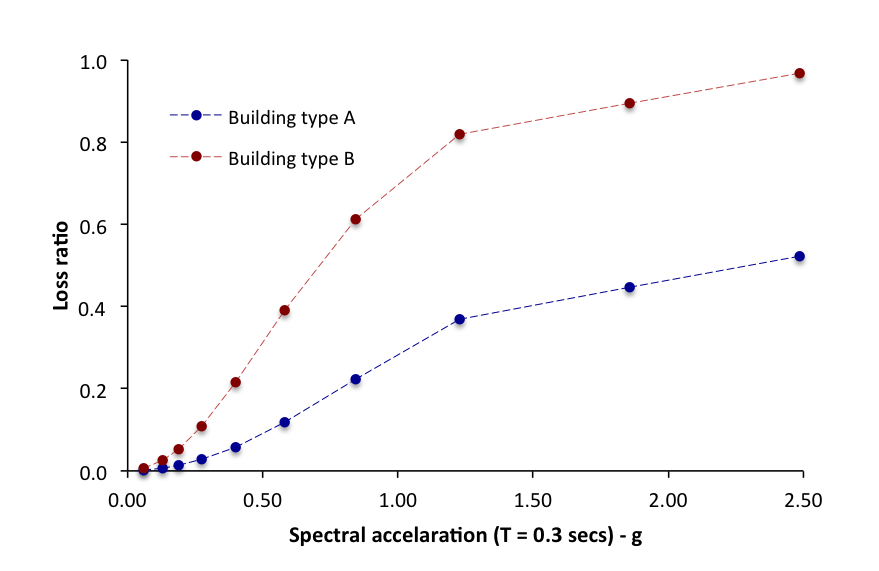
\includegraphics[width=10cm,height=6cm]{./oqum/figures/vulnerabilityModel.eps}
\caption{Graphical representation of a vulnerability model.}
\label{fig:vulModel}
\end{figure}

Each component of the associated NRML file is presented herein:

\begin{Verbatim}[frame=single, commandchars=\\\{\}, samepage=true]
<\textcolor{red}{vulnerabilityModel}>
    <\textcolor{green}{discreteVulnerabilitySet} vulnerabilitySetID="OpenQuake2011"	
    assetCategory="buildings"    lossCategory="economic loss">
        ...
\end{Verbatim}

At the top of the NRML schema, the following metadata are being stored:
\begin{itemize}
\item  \Verb+vulnerabilitySetID+: A unique key used to identify the vulnerability model instance within OpenQuake;
\item  \Verb+assetCategory+: An attribute that describes the asset typology (e.g.: population, buildings, contents);
\item  \Verb+lossCategory+: An attribute that describes the type of loss suffered by the assetCategory (e.g.: fatalities, collapse, economic loss). 
\end{itemize}

\begin{Verbatim}[frame=single, commandchars=\\\{\}, samepage=true]
    ...
        <\textcolor{blue}{IML}  IMT = "Sa 0.3"> 0.061 0.129 0.188 0.273 0.398 0.579 
        0.843 1.227 1.856 2.485 <\textcolor{blue}{/IML}>
        ...
\end{Verbatim}

Within this component, an attribute specifying the intensity measure type (e.g.: Sa, PGA, MMI) is defined, followed by the list of intensity measure levels. This set of values is common to all of the vulnerability functions.

\begin{Verbatim}[frame=single, commandchars=\\\{\}, samepage=true]
        ...
        <\textcolor{blue}{discreteVulnerability}  vulnerabilityFunctionID="typeA" 
        probabilisticDistribution="LN">
            <\textcolor{magenta}{meanLossRatio}> 0.002 0.007 0.014 0.028 0.058 0.118
            0.223 0.370 0.446 0.523 <\textcolor{magenta}{/meanLossRatio}>
            <\textcolor{magenta}{coefficientVariation}> 0.012 0.058 0.079 0.159 0.265 
            0.244 0.211 0.152 0.088 0.082 <\textcolor{magenta}{/coefficientVariation}>
        <\textcolor{blue}{/discreteVulnerability}>
        <\textcolor{blue}{discreteVulnerability}  vulnerabilityFunctionID="typeB" 
        probabilisticDistribution="LN">
            <\textcolor{magenta}{meanLossRatio}> 0.006 0.025 0.052 0.108 0.215 0.391	
            0.613 0.820 0.894 0.967 <\textcolor{magenta}{/meanLossRatio}>
            <\textcolor{magenta}{coefficientVariation}> 0.010 0.054 0.082 0.167 0.285 
            0.278 0.261 0.132 0.084 0.021 <\textcolor{magenta}{/coefficientVariation}>
        <\textcolor{blue}{/discreteVulnerability}>
    <\textcolor{green}{/discreteVulnerabilitySet} 
<\textcolor{red}{/vulnerabilityModel}>        
\end{Verbatim}

Finally, for each discrete vulnerability function the following parameters are required:
\begin{itemize}
\item  \Verb+ vulnerabilityFunctionID +: A unique key that is used to relate each vulnerability function with the exposure elements;
\item  \Verb+ probabilisticDistribution +: An attribute that establishes the type of probabilistic distribution followed by the loss ratio uncertainty. At the moment, OpenQuake only supports lognormal distributions, however, other types of distributions such as beta will be incorporated in future releases;
\item  \Verb+ meanLossRatio +: A set of loss ratios (one per each intensity measure level defined previously). These values can represent different losses such as fatality rates (quotient between the number of fatalities and total population exposed) or damage ratio (quotient between the repair cost and the replacement cost of a given structure).
\item  \Verb+ coefficientVariation +: A set of coefficients of variation (one per loss ratio) that describes the uncertainty for different levels of loss. If users do not want to consider the uncertainty, this set of parameters can be set to zero, and OpenQuake assumes each loss ratio as a deterministic value. 
\end{itemize}

Several methodologies to derive vulnerability functions are currently being evaluated and will be a part of the Modelers Toolkit. In addiction, scripts to convert vulnerability curves stored in Excel or ASCII files into NRML are being developed.
